\chapter{Conclusion}\label{conclusion}

\section{Bilan de notre travail de groupe}
Le broadcast est primordiale dans les réseaux de capteur sans fils. Dans ce TER, nous avons présenté le probleme, puis établi un cadre 
formel nous permettant de presenter et de simuler quelques algorithmes. 



Le bilan de notre travail en groupe est assez simple. Il a été planifié par le diagramme de GANTT qu'on a élaboré au tout début.

\begin{figure}[tb]
    \centering
    \begin{tabular}{cccc}
      
      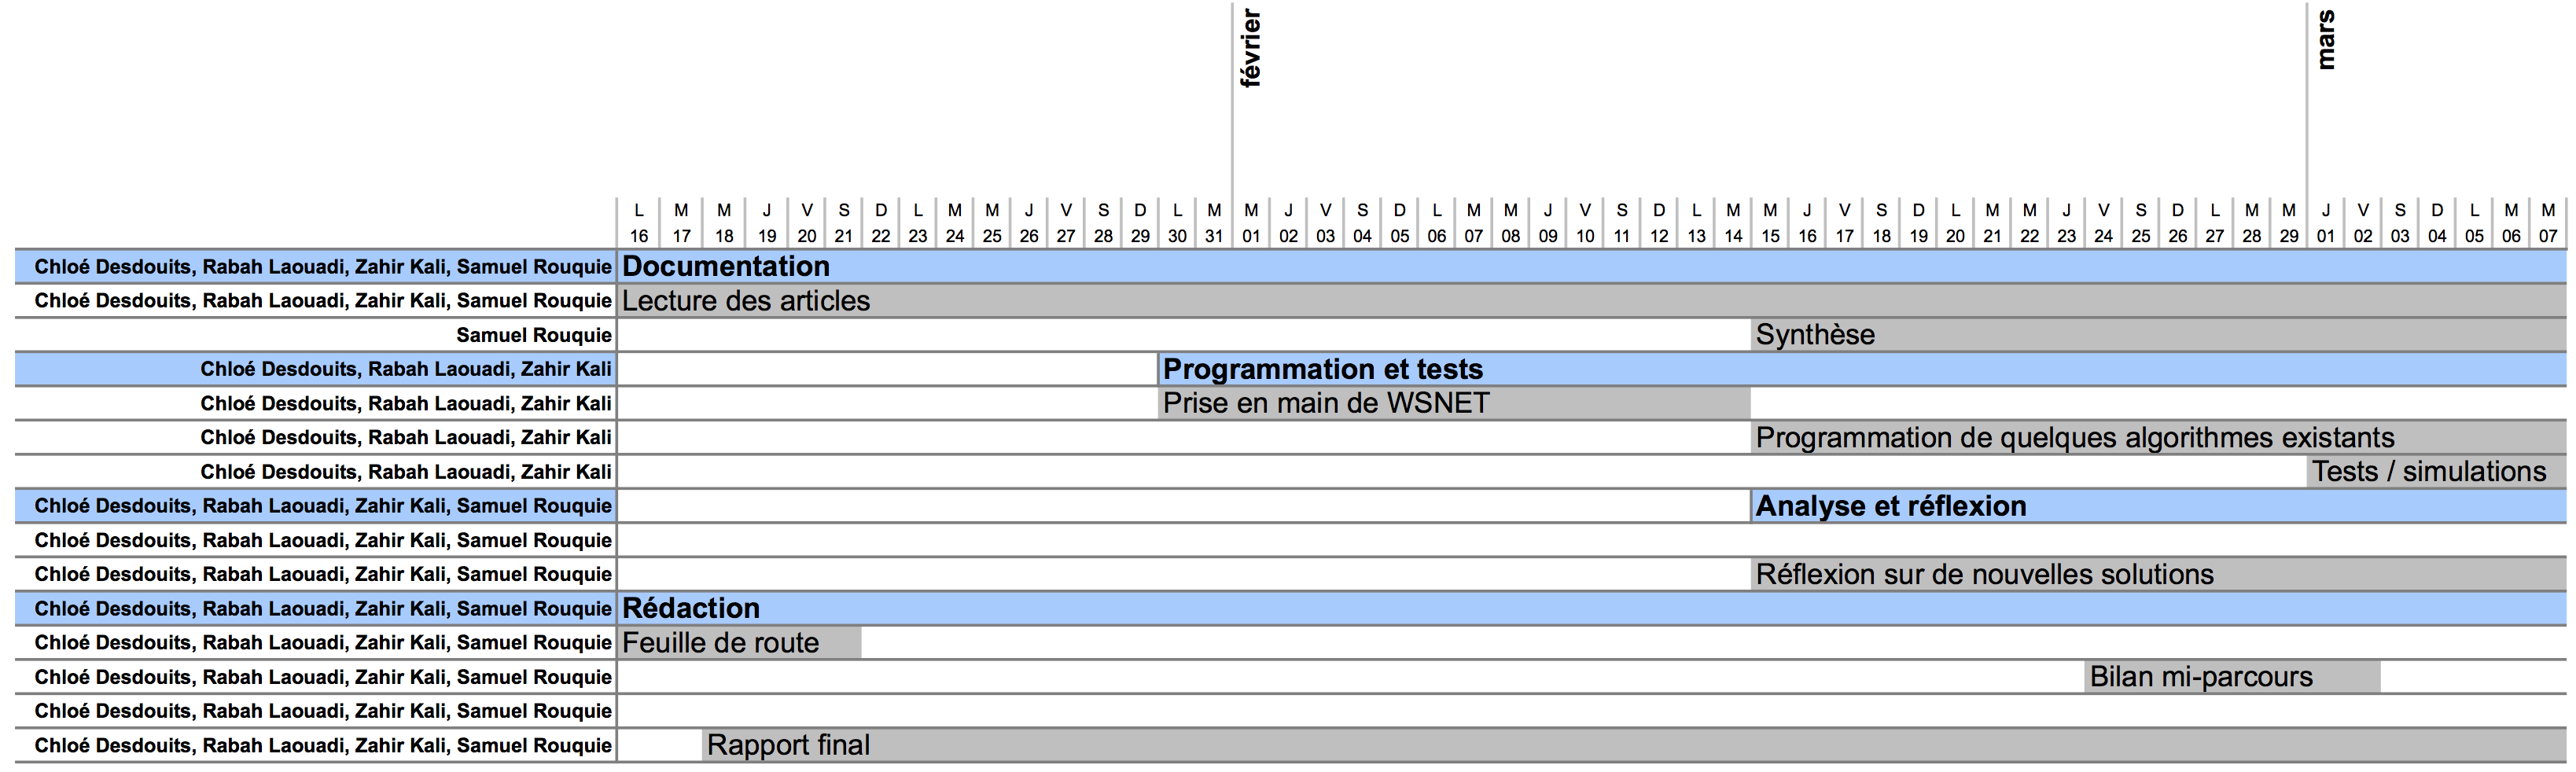
\includegraphics[angle=90, scale= 0.5,width=.5\linewidth]{Conclusion/diagramme} &
      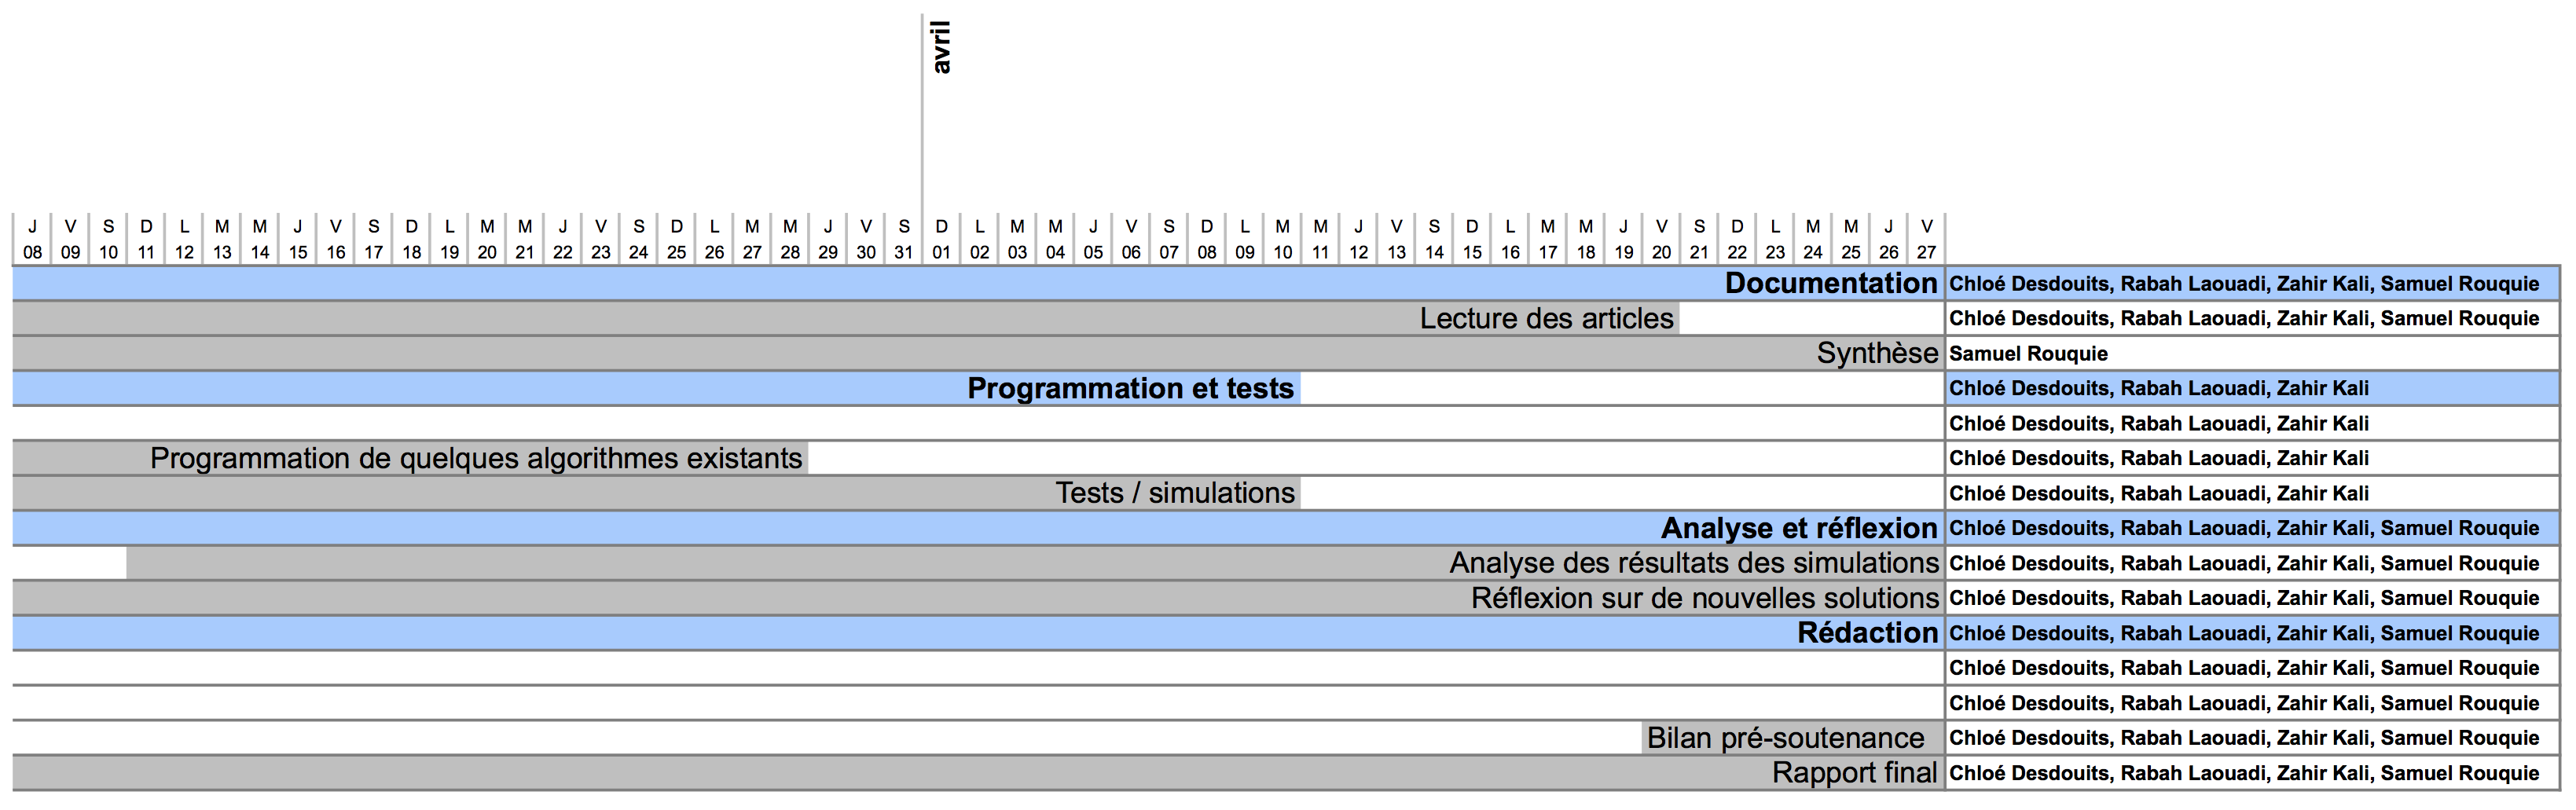
\includegraphics[angle=90, scale= 0.5,width=.5\linewidth]{Conclusion/diagramme2} 
   \\
      (a) & (b) \\
    \end{tabular}
    \caption{Graphe Unité(a) et Graphe Disque(b) \label{Unit}}
\end{figure}

Au debut du travail, nous nous sommes entendus que chacun fasse des recherches sur le sujet de son coté en lisant 
deux articles, puis nous avons constitué 2 sous-groupes, le premier qui commencait la programmation et le second 
s'approfondit dans les recherches. Etant satisfaits de l'avancement de la programmation, on a décidé de diminuer 
le nombre de programmeurs pour permettre en meme temps d'avancer sur la rédaction du rapport.

Pour le bon déroulement de notre travail, nous avons utilisé le GIT comme moyen de collaboration, ceci s'ajoute 
aux réunions régulières qu'on organise pratiquement une fois par semaine.

Durant notre travail, nous avons rencontré quelques problèmes dûs à l'ambiguité du thème, et ceci particulièrement
dans la désignation des choix des algorithmes qui convergent le plus vers notre sujet. Ceci s'ajoute à la difficulté 
de la prise en main du GIT puisque la moitié du groupe n'y était pas familliarisé.

\section{Bilan du TER}

Le broadcast est primordiale dans les réseaux de capteur sans fils. Dans ce TER, nous avons présenté le probleme, puis établi un cadre 
formel nous permettant de presenter et de simuler quelques algorithmes. 
